\documentclass[conference]{IEEEtran}

% ---------- Packages ----------
\usepackage{newtxtext,newtxmath} % Times系/数式(amssymb不要)
\usepackage{amsmath}             % ← amssymb は読み込まない
\usepackage{siunitx}
\usepackage{graphicx,xcolor}
\usepackage{booktabs}
\usepackage{placeins}
\usepackage[hidelinks]{hyperref}

\usepackage{tikz}
\usetikzlibrary{calc,positioning,fit,arrows.meta,shapes.geometric,shapes.misc}

% ---------- TikZ styles ----------
\tikzset{
  line/.style={-Latex, line width=0.4pt},
  box/.style={draw, rounded corners, align=center, inner sep=3pt},
  smallbox/.style={box, minimum width=28mm, minimum height=7mm},
  midbox/.style={box, minimum width=34mm, minimum height=8mm},
  bigbox/.style={box, minimum width=68mm, minimum height=9mm}
}

% ---------- Title ----------
\title{AITL on Space: A Robust Three-Layer Architecture\\
with a Tri-NVM Hierarchy (SRAM / MRAM / FRAM)\\
for Long-Duration Spacecraft Autonomy}

\author{
\IEEEauthorblockN{Shinichi Samizo}
\IEEEauthorblockA{Independent Semiconductor Researcher\\
Former Engineer at Seiko Epson Corporation\\
Email: shin3t72@gmail.com\quad GitHub: \url{https://github.com/Samizo-AITL}}
}

\begin{document}
\maketitle

\begin{abstract}
We propose \emph{AITL on Space}, a three-layer control architecture (Robust Core, FSM Supervisor, AI Adaptor) implemented on a 22\,nm FD\!SOI SoC with a hardened tri-NVM hierarchy (SRAM/MRAM/FRAM). The system targets ultra-robust autonomy under radiation, thermal cycling, and long-term drift. This paper outlines the architecture, an 11D state-space plant model (8--20D extensible), an $H_\infty$ mixed-sensitivity design flow, and a verification pipeline from FPGA HIL to ASIC.
\end{abstract}

\section{Introduction}
Long-duration missions require high availability under total ionizing dose (TID), single event effects (SEE), and thermal cycling. Conventional PID\,+\,Flash architectures face reliability limits due to charge-trap drift and write endurance. We summarize related work and motivate AITL on Space as a resilient alternative.

\section{System Architecture}
AITL comprises three layers:
\begin{itemize}
  \item \textbf{Robust Core} for $H_\infty$/MPC/SMC control,
  \item \textbf{FSM Supervisor} (Safe/Nominal/Recovery; FDI/FDII),
  \item \textbf{AI Adaptor} for long-term re-identification and drift compensation.
\end{itemize}
A tri-NVM hierarchy is adopted: SRAM for execution, MRAM for code/logs (ECC\,+\,scrub, A/B slots), and FRAM for safe boot and FSM state. The target implementation is a 22\,nm FD\!SOI SoC hardened for radiation and temperature cycling.

% ---------- Fig.1 Architecture ----------
\begin{figure*}[t]
\centering
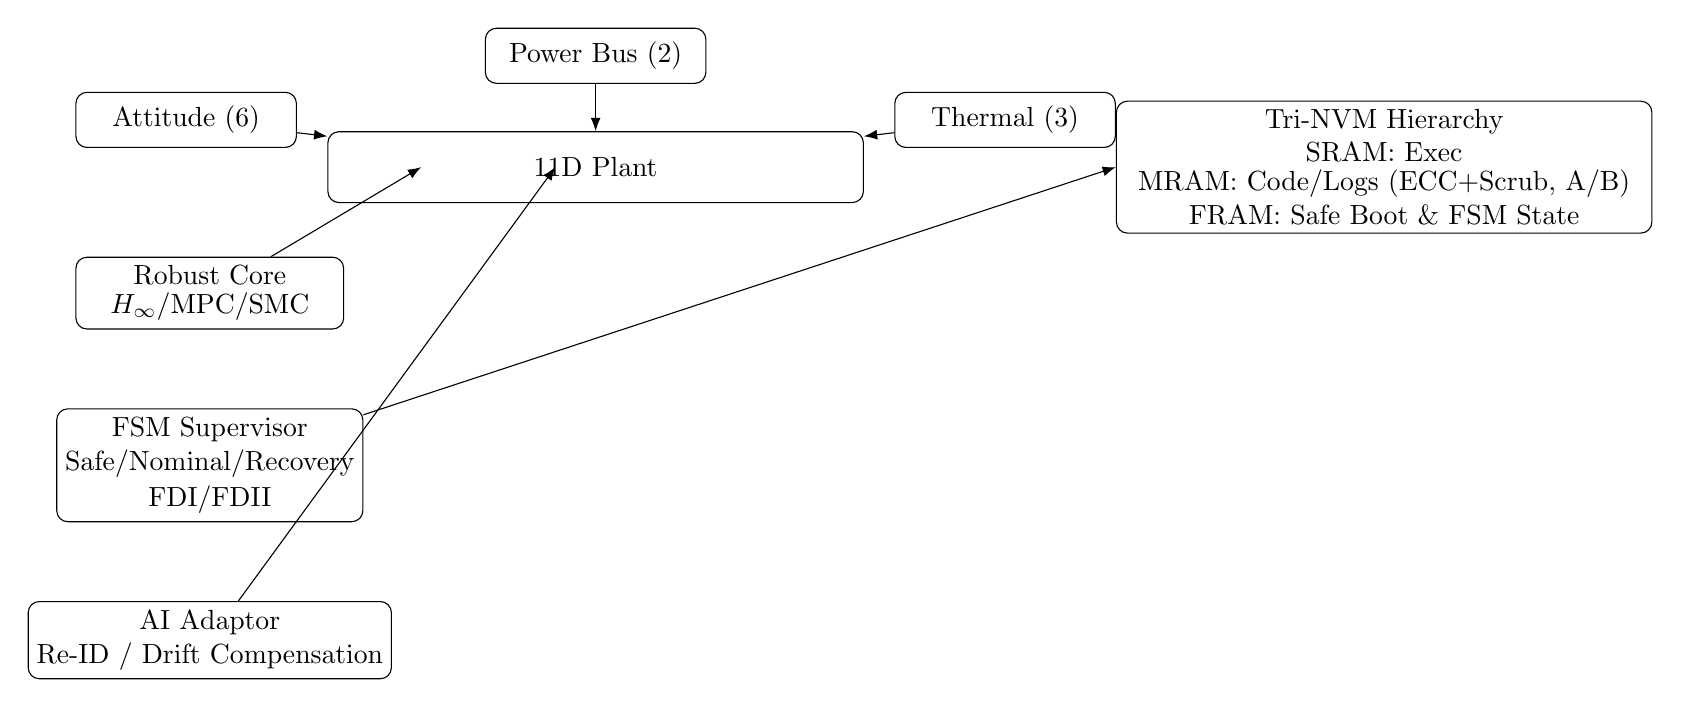
\begin{tikzpicture}[node distance=6mm]
  % plant
  \node[bigbox] (plant) {11D Plant};
  \node[smallbox, above left=6mm and 0mm of plant.west, anchor=west, xshift=-32mm] (att) {\shortstack{Attitude (6)}};
  \node[smallbox, above=6mm of plant.east, anchor=east, xshift=32mm] (therm) {\shortstack{Thermal (3)}};
  \node[smallbox, above=6mm of plant, xshift=0mm] (bus) {\shortstack{Power Bus (2)}};

  % left column
  \node[midbox, below=16mm of plant.west, anchor=west, xshift=-32mm] (core)
     {\shortstack{Robust Core\\$H_\infty$/MPC/SMC}};
  \node[midbox, below=10mm of core] (fsm)
     {\shortstack{FSM Supervisor\\Safe/Nominal/Recovery\\FDI/FDII}};
  \node[midbox, below=10mm of fsm] (ai)
     {\shortstack{AI Adaptor\\Re-ID / Drift Compensation}};

  % tri-NVM
  \node[bigbox, right=32mm of plant] (nvm) {\shortstack{Tri-NVM Hierarchy\\
    SRAM: Exec\\MRAM: Code/Logs (ECC+Scrub, A/B)\\FRAM: Safe Boot \& FSM State}};

  % arrows
  \draw[line] (core) -- ($(plant.west)!0.35!(plant.center)$);
  \draw[line] (fsm) -- (nvm.west);
  \draw[line] (ai) -- ($(plant.west)!0.85!(plant.center)$);
  \draw[line] (att) -- (plant);
  \draw[line] (bus) -- (plant);
  \draw[line] (therm) -- (plant);
\end{tikzpicture}
\caption{AITL on Space architecture with Robust Core, Supervisor FSM, AI Adaptor, and the Tri-NVM hierarchy.}
\label{fig:arch}
\end{figure*}

\section{Mathematical Model}
We use an 11D discrete-time plant that couples attitude (6), power bus (2), and thermal nodes (3):
\begin{align}
  x_{k+1} &= A x_k + B u_k + E w_k, \label{eq:ss1}\\
  y_k &= C x_k + D u_k + v_k. \label{eq:ss2}
\end{align}
The model extends to 20D by adding translational axes and bias states. $w_k$ and $v_k$ represent disturbance and sensor noise, respectively.

% ---------- Fig.2 Control loop ----------
\begin{figure}[t]
\centering
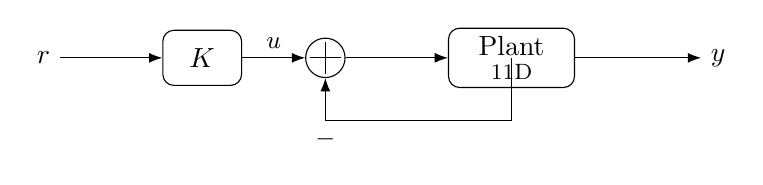
\begin{tikzpicture}[node distance=10mm]
  \node[smallbox, minimum width=10mm] (K) {$K$};
  \node[circle, draw, minimum size=5mm, right=8mm of K] (sum) {};
  \draw (sum) +(-2mm,0) -- +(2mm,0);
  \draw (sum) +(0,-2mm) -- +(0,2mm);
  \node[smallbox, right=13mm of sum, minimum width=16mm] (P) {\shortstack{Plant\\\footnotesize 11D}};
  \node[right=16mm of P] (y) {$y$};
  \node[left=13mm of K] (r) {$r$};
  \draw[line] (r) -- (K);
  \draw[line] (K) -- node[above]{\small $u$} (sum);
  \draw[line] (sum) -- (P);
  \draw[line] (P) -- (y);
  \draw[line] ($(P.north)!0.5!(P.south)$) |- ++(0,-8mm) -| node[below]{\small $-$} (sum.south);
\end{tikzpicture}
\caption{Closed-loop schematic used for $H_\infty$ synthesis on the 11D plant.}
\label{fig:loop}
\end{figure}

\section{\texorpdfstring{$H_\infty$}{H-infinity} Mixed-Sensitivity Design}
Weights $(W_1,W_2,W_3)$ shape sensitivity, control effort, and complementary sensitivity, respectively. A teaching controller (\texttt{EduController}) exports JSON plant/weights; AITL-H synthesizes an output-feedback $K$ and a fixed-point realization suitable for FPGA/ASIC.

\section{Verification Pipeline}
FPGA HIL injects SEU bursts and sensor outages; metrics include safe-mode time ($<\SI{1}{s}$), recovery rate ($\ge\SI{99}{\percent}$), and ECC statistics during scrubbing. Physical design proceeds to 22FDX tape-out; SystemDK FEM closes thermal/packaging effects with radiation/temperature scenarios.

% ---------- Fig.3 Flow ----------
\begin{figure}[t]
\centering
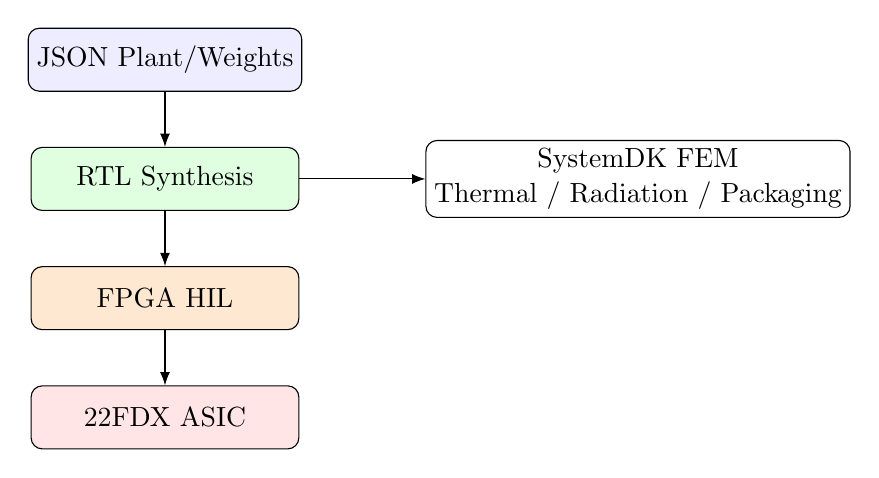
\begin{tikzpicture}[node distance=7mm]
  \node[midbox, fill=blue!7] (json) {JSON Plant/Weights};
  \node[midbox, fill=green!12, below=of json] (rtl) {RTL Synthesis};
  \node[midbox, fill=orange!18, below=of rtl] (hil) {FPGA HIL};
  \node[midbox, fill=red!10, below=of hil] (asic) {22FDX ASIC};

  \node[midbox, right=16mm of rtl] (fem) {\shortstack{SystemDK FEM\\Thermal / Radiation / Packaging}};

  \draw[line] (json) -- (rtl);
  \draw[line] (rtl) -- (hil);
  \draw[line] (hil) -- (asic);
  \draw[line] (rtl) -- (fem);
\end{tikzpicture}
\caption{Verification pipeline from JSON design to RTL, FPGA HIL, and ASIC; FEM closes the loop with thermal and radiation scenarios.}
\label{fig:flow}
\end{figure}

\section{Conclusion}
AITL on Space provides a practical path to resilient autonomy for deep-space missions by combining robust control, supervisory safety logic, AI-based re-identification, and a tri-NVM memory hierarchy.

% ---------- References ----------
\begin{thebibliography}{99}
\bibitem{doyle}
J.\,C.~Doyle, B.\,A.~Francis, and A.\,R.~Tannenbaum,
\emph{Feedback Control Theory}. Macmillan, 1992.

\bibitem{colinge}
J.-P.~Colinge, \emph{Silicon-on-Insulator Technology: Materials to VLSI}, 3rd~ed. Springer, 2004.
\end{thebibliography}

% ---------- Biography ----------
\section*{Author Biography}
Shinichi Samizo received the M.S.\ degree in Electrical and Electronic Engineering from Shinshu University, Japan. He worked at Seiko Epson Corporation as an engineer in semiconductor memory and mixed-signal device development, and contributed to inkjet MEMS actuators and PrecisionCore printhead technology. He is currently an independent semiconductor researcher focusing on process/device education, memory architecture, and AI system integration. Contact: \texttt{shin3t72@gmail.com}.
\end{document}
